\begin{figure}[t]
\centering
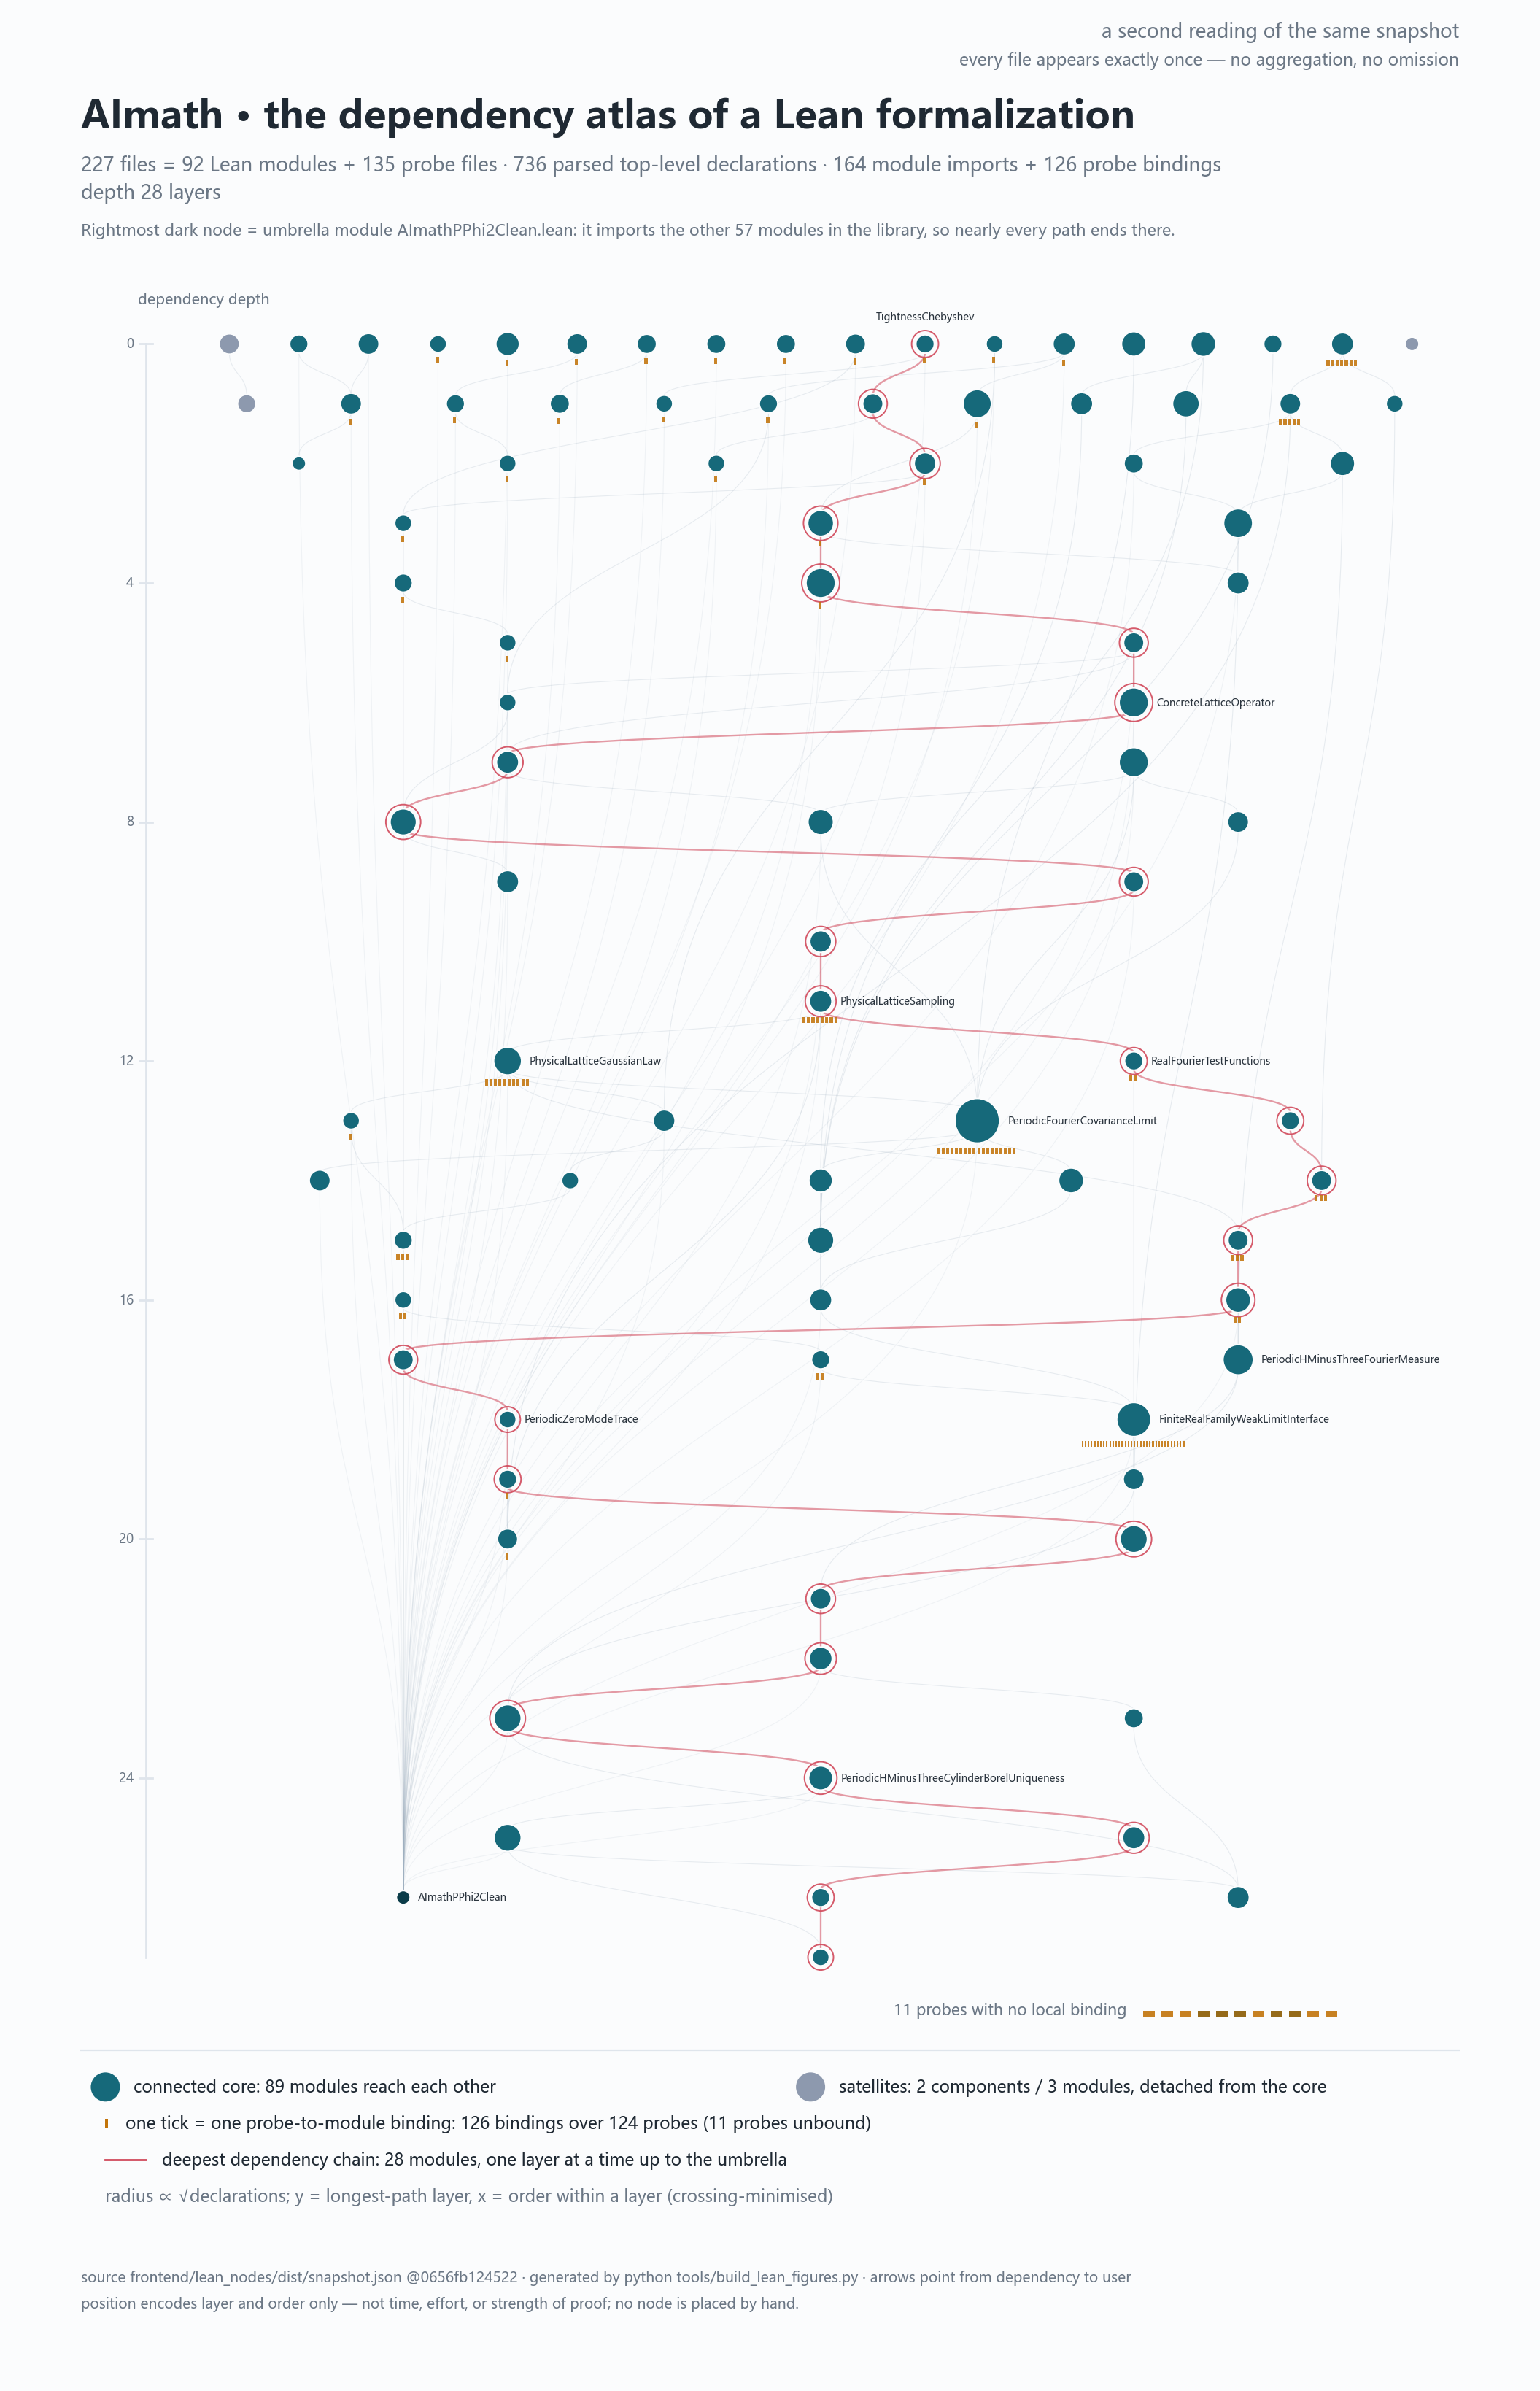
\includegraphics[width=0.62\linewidth]{figures/lean_atlas_en_portrait.png}
\caption{Dependency atlas of the Lean development. Each node is a module and each edge a declaration dependency. The atlas is a snapshot of a slightly wider tree than the package of \cref{sec:lean-overview}: it reports $92$ modules and $135$ probe files against the package's \NumCleanModules{} and \NumAuditProbes, and the figure's own legend identifies the three extra modules as satellites detached from the core rather than as part of it. The dense core the atlas names is the package. The surrounding directory of \cref{sec:lean-overview} is much larger than either count --- it holds \NumRootFiles{} further modules --- and none of it is drawn here. The figure is therefore best read as a picture of where the reported chain sits inside the tree that was measured, not as evidence about anything outside that chain.}
\label{fig:atlas}
\end{figure}
